\documentclass[12pt, a4paper, oneside,UTF8]{ctexart}
\usepackage{amsmath, amsthm, amssymb, bm, color, framed, graphicx, hyperref, mathrsfs,amsfonts}
\usepackage[left=1.0cm,right=1.0cm,top=1.5cm,bottom=1.5cm]{geometry}
\usepackage{booktabs,multirow,tabularray}%表格使用,转换使用excel插件
\usepackage{pgf-pie}%饼图使用
%\linespread{1.5}
\definecolor{shadecolor}{cmyk}{0.09,0.63,0,0.51}
% \definecolor{NJUblue}{cmyk}{0.09,0.63,0,0.51}
\newcounter{problemname}
\newenvironment{problem}{\stepcounter{problemname}\par\noindent\textbf{题目\arabic{problemname}. }}{\par}
\newenvironment{solution}{\begin{shaded}\par\noindent\textbf{解答. }}{$\Box$\end{shaded}\par}
\newenvironment{note}{\par\noindent\textbf{题目\arabic{problemname}的注记. }}{\par}
\ctexset{ section = { format={\Large \bfseries } } }
\DeclareMathOperator{\st}{s.t.}
\renewcommand{\familydefault}{\rmdefault} %可选择\rmdefault \sfdefault \ttdefault 分别是罗马字体,sans-serif字体和等宽字体  \familydefault是默认字体

\title{标题}
\author{李冠霖 221502012}
\date{\today}
\begin{document}
\maketitle
\tableofcontents
\newpage
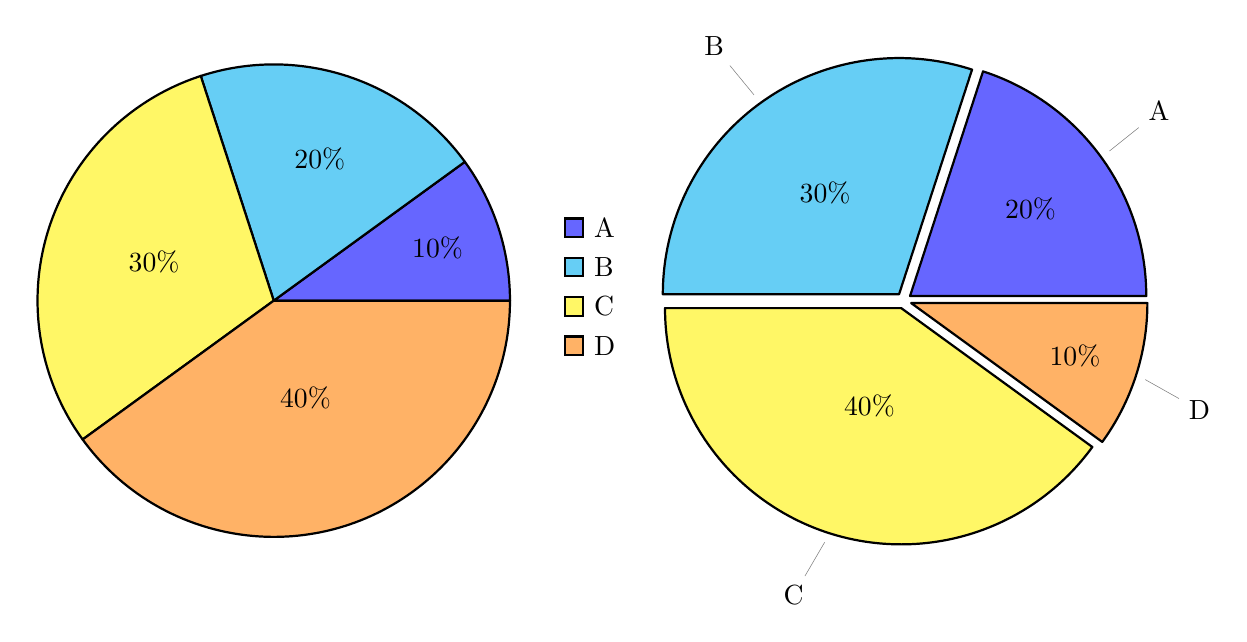
\begin{tikzpicture}
    \pie[text=legend]{10/A, 20/B, 30/C, 40/D}
    \pie[text=pin,pos={8,0},explode=0.1]{20/A, 30/B, 40/C, 10/D}
\end{tikzpicture}
\bibliography{ref}
\bibliographystyle{alpha}
\end{document}